\documentclass{paper}
\usepackage[utf8]{inputenc}
\usepackage{amsmath,amssymb,amsthm}
\usepackage{glossaries}
\usepackage[ruled,vlined]{algorithm2e}
\usepackage[most]{tcolorbox}
\usepackage{hyperref}
\usepackage{lmodern}
\newlength\longest



\newenvironment{wexample}[2][Worked example:]{\begin{trivlist}
\item[\hskip \labelsep {\bfseries #1}\hskip \labelsep {\bfseries #2.}]}{\end{trivlist}}

\newenvironment{aside}[2][Aside:]{\begin{trivlist}
\item[\hskip \labelsep {\bfseries #1}\hskip \labelsep {\bfseries #2.}]}{\end{trivlist}}

\newenvironment{solution}{\begin{proof}[Solution]}{\end{proof}}

\newenvironment{ybox}{\begin{tcolorbox}[breakable,colback=yellow!20!white,colframe=brown!100!black]}{\end{tcolorbox}}

\newenvironment{gbox}{\begin{tcolorbox}[breakable,colback=green!20!white,colframe=green!10!black]}{\end{tcolorbox}}

\title{Hill Ciphers: A Measured Perspective}
\author{Alex Rankine }
\date{December 2020}

\begin{document}

\maketitle

Imagine that you're Bob, an undercover cop living in early 1930s America, and you wish to mail a message communicating the location of a large stash of bootleg liquor to your supervisor Alice in the next town over. However, corruption is rife, and the gang selling the liquor on the black market also happens to control the mail center. If they happen to understand your message, they'll move the stash to another location within the hour, making all those hours of surveillance for naught. You also have the benefit of knowing that the top crime boss Joe happens to an amateur cryptographer! 

\medskip
So a simple Caesar or Vigenère cipher unfortunately won't stop him from reading your message. Stumped for ideas, you browse through the June edition of \textit{The American Mathematical Monthly}, a journal that Alice also happens to read quite a bit. Flipping through the pages, one article catches your eye: "Cryptography in an Algebraic Alphabet", written by a Lester S. Hill of Hunter College.

\medskip
After reading through the paper, you take your pen to a scrap of paper and write the following string of letters 

\[ \mathrm{GYBNQKURP} \]

alongside the string

\[ \mathrm{PIQIZAWVZZQDCCWJXTUNALNK} \]

Last but not least, you draw a crude picture of a snow-capped hill at the bottom of the paper, hoping that Alice will get the hint. You stuff your hastily-written message into an envelope and drop it in the mail box. A few days later, you receive a manila envelope from Alice containing only a crisp, eggwhite sheet of paper with the neatly-typed letters

\[ \mathrm{EKGKIIUANMOURDNFSXWTNSZQPMTLNK} \]

What do either of these strings mean? Did the meaning of your message in fact manage to slip by Joe's inquisitive eyes? Or has he and his illicit cache of moonshine already vanished, never to see the light of justice evermore? To answer these questions, we must start at beginning.

\newpage

\tableofcontents

\clearpage

\thispagestyle{empty}
\null\vfill

\settowidth\longest{\huge\itshape just as his inclination leads him;}

\begin{center}
    \parbox{\longest}{%
  \raggedright{\Large\itshape%
   The enemy knows the system. \par\bigskip
  }   
  \raggedleft\MakeUppercase{Claude Shannon}\par%
}

\end{center}


\vfill\vfill

\clearpage


\part{Cryptography, expedited}

Mathematics is said to be the logic of certainty\footnote{According to \href{https://twitter.com/stat110/status/288032140728365059?s=20}{Joe Blitzstein}, at least}. In some ways, cryptography is the logic of trying to make the certain appear uncertain. It should seem that the two are incompatible, but nothing is farther from the truth. 

\medskip

Cryptography is the practice of enabling secure communication via the use of \textbf{ciphers}, algorithms that convert plaintext (i.e. text we can understand) to ciphertext (i.e. text we do not readily understand) and back again. Ciphers typically rely on some \textbf{key}, a crucial piece of information that allows senders and receivers to encrypt and decrypt messages respectively.

\medskip
When designing ciphers, we're especially concerned with the question of whether they're robust to \textbf{cryptanalysis}; that is, methods of deciphering the ciphertext \textit{without} explicit knowledge of the key. As we'll see, it can be challenging to design ciphers that are hard to cryptanalyze.

\section{Classical cryptography}

Cryptography has been around as long as people have sought to conceal information from one another. Naturally, the field has progressed to a state where ciphers today are quite advanced, often requiring nontrivial background in number theory and probability to grasp. We'll only concern ourselves with classical cryptography, which is primarily organized around two approaches to enciphering text: \textbf{substitution} and \textbf{transposition}.

\medskip Substitution ciphers encrypt text by substituting letters with other letters in a systematic manner, whereas transposition ciphers operate by instead transposing the order of the given letters. Here we'll mostly focus on the former with an example.

\subsection{A cryptographic classic: the Caesar cipher}

The Caesar cipher is a simple substitution cipher, rumored to have been used by the eponymous Julius Caesar to encrypt messages of great tactical import during his many military campaigns. The steps for encrypting a message with a Caesar cipher are formalized in Algorithm 1, but the main idea is to choose some natural number $k$ as our key, map each letter in our alphabet $\Sigma$ to some number between $0$ and $|\Sigma|$. In Algorithm 1, the alphabet is simply $\Sigma = \{ a, b, c, \dots, x, y, z \}$, but one can easily extend this to alphabets other than the Latin one.

\begin{algorithm}
    \SetAlgoLined
    \KwData{A plaintext string of $n$ letters $x = x_0, \dots, x_{n - 1}$, represented as numbers between 0 and 25 (i.e. $A \mapsto 0, B \mapsto 1, \dots$)}
    \KwResult{The ciphertext of $n$ letters $c = c_0, \dots, c_{n-1}$ and a key $k$}
    Choose a key $k \in \mathbb{N}$\;
    \For{every letter $x_i \in x$}{
        $c_i \gets (x_i + k) \bmod 26$\;
    }
    return $(c_0, \dots, c_{n-1}), k$\;
    \caption{Caesar cipher; encrypting}
\end{algorithm}

\medskip
We then take the numeric value of each character $x_i$, add $k$ to it, and take the result modulo\footnote{If you're not familiar with modular arithmetic, for our purposes you can think of the expression $a \mod b$ as the remainder of dividing $a$ by $b$. We read this expression as "$a$ modulo $b$". When dealing with modular arithmetic, we might perform common operations like addition or multiplication "modulo $b$", which can be likened to performing the operation first and then taking the result modulo $b$.} $|\Sigma|$ as $c_i$, the substituted letter in our ciphertext. The resulting string $c$ is our ciphertext. 

\medskip
Decrypting our ciphertext back to plaintext is also easy: we recover $x_i$ by subtracting $k$ from the numeric value of $c_i$ and taking the result modulo $26$ once more. Crucially, this relies on knowing what choice of $k$ we made during the encryption process. This necessitates that whoever's sending and receiving the message agree on what $k$ is ahead of time. 

\bigskip
\begin{ybox}
    \begin{wexample}{Encrypting using a Caesar cipher}
        Say $k = 10$, and we wish to encipher the plaintext "retreatatdawn". What should the resulting ciphertext be?
    \end{wexample}
    \begin{solution}
        We perform the cipher for the first letter only. Using the mapping $a \mapsto 0, b \mapsto 1, \dots$, we see that $r \mapsto 17$. By going through the arithmetic, we see that 
        
        \begin{equation*}
            \begin{split}
            c_i & = (17 + 10) \bmod 26 \\
             & = 27  \bmod 26 \\
             & = 1
            \end{split}
        \end{equation*}
        
        and so the letter to be substituted in for $r$ is thus $b$. If we were the receiver, we could recover $r$ from $b$ as by subtracting key $k$ instead:
        
        \begin{equation*}
            \begin{split}
            c_i & = (1 - 10) \bmod 26 \\
             & = -9 \bmod 26 \\
             & = 17
            \end{split}
        \end{equation*}
    \end{solution}
    
     We leave it as an exercise to the reader to verify that the complete ciphertext is "bodbokdkdnkgx".
\end{ybox}

\subsection{Cracking Caesar}

\medskip Note that if $k = 0$, then our cipher makes no substitutions whatsoever and wouldn't be much of a cipher at all. In fact, if $k \mod |\Sigma| = 0$, then the cipher is still trivial. This follows from the identity 
\begin{equation}
    (a + b) \bmod c = (a \bmod c) + (b \bmod c)
\end{equation}
since then we have for any $x_i \in \Sigma$
\begin{equation*}
    \begin{split}
    c_i & = (x_i + k) \bmod |\Sigma| \\
     & = (x_i \bmod |\Sigma|) + (k \bmod |\Sigma|) \\
     & = x_i 
    \end{split}
\end{equation*}

Although this poses quite the constraint on our choice of $k$, you may think because that our \textbf{keyspace}--that is, the set of all possible keys $k$--is still infinitely big, there are infinitely many Caesar ciphers! Unfortunately, it turns out there's only as many Caesar ciphers as there are characters in our alphabet, which follows the observation that $(x_i + k +  |\Sigma|) \bmod |\Sigma| = (x_i + k) \bmod |\Sigma|$. 

\medskip
As an example, say $k = 1$ and we're again working with our familiar Latin alphabet, such that $|\Sigma| = 26$. Then, let's say we want to substitute $x_i =$ 'c'. Then, we obtain that $c_i = 3 =$ 'd', as
\[ c_i = (2 + 1) \bmod 26 = 3 \]
but we just as well could've chosen $k = 27$, as $(2 + 27) \bmod 26 = 3$. Or $k = 53$. Primarily for this reason, the Caesar cipher is not robust to cryptanalysis. If we knew that some ciphertext was encrypted using a Caesar cipher\footnote{The idea that "the enemy knows the system" is a common assumption in cryptanalysis. Any adversaries trying to break a cipher may have full knowledge of how the cipher works, but we can assume they don't know the key.}, then we need only test $|\Sigma|$ possible keys when trying to decrypt it. Perhaps a Gallic codebreaker would've had trouble doing this, but it's trivial for modern computers.

\medskip
This practice of performing an exhaustively searching all the keys and subjecting the cipher to a \textbf{brute-force attack} is only one way to break a cipher. It turns out there are even more efficient ways to break a Caesar Cipher, given a little information. In particular, say we knew that for some Caesar cipher that it substitutes the letter $e$ with the letter $n$. Then, we can solve for the key $k$ by observing that 

\begin{equation*}
    \begin{split}
    13 & = (4 + k) \bmod 26 \\
    13 & = (4 \bmod 26) + (k \bmod 26) \\
    13 & = 4 + (k \bmod 26) \\
    9 & = (k \bmod 26) \\
    k & = 9
    \end{split}
\end{equation*}

You may object to our assumption of knowing that $b$ is substituted by $n$, but in practice it is easy to guess which letters are substituted by which letters through the use of \textbf{frequency analysis}. This technique compares the frequencies of letters in the ciphertext with the frequencies of letters in the chosen language to make educated guesses about which cipher letters correspond to which plain letters. 

\medskip
As an informal example of this, we know that the letter $e$ is the one of the most common letters in English. In the ciphertext "ancanjcjcmjfw", the letters $n$, $j$, and $c$ appear quite frequently, so we can individually test a few assumptions like $n \mapsto e$, $j \mapsto e$, or $c \mapsto e$ and find that only the assumption that $n \mapsto e$ produces intelligible text\footnote{Of course, it's possible that there are multiple keys that would reverse the ciphertext back into something intelligible, but in unlikely event that this happens in practice, the "true" message can inferred from context, i.e. who's sending the message, who's receiving it, what they're likely to talk about, $\dots$}, so the key is probably $9$.

\newpage

\part{The Hill Cipher}

You may be wondering how our discussion of Caesar ciphers relates at all to the mystery in the exposition. The Caesar cipher is one example of a \textbf{monographic substitution cipher}, "monographic" meaning that only individual letters are substituted, as opposed to groupings of those letters. But it's not hard to envision the concept of \textbf{polygraphic substitution ciphers}, where blocks of $n$ letters are substituted with other blocks of $n$ letters. Unlike the letter-to-letter bijection we saw with Caesar ciphers, here the cipherletter that some plainletter gets mapped to depends on the identity of the $n - 1$ plainletters in its block.

\medskip
The cipher featured in the exposition is a polygraphic substitution cipher known as the \textbf{Hill cipher}, attributed to the aforementioned Lester Hill. It distinguishes itself from simpler substitution ciphers like the Caesar cipher since it's founded on several ideas from linear algebra. We'll familiarize ourselves with them through an example.

\section{Jekyll's ruin}

Mr. Hyde wishes to send the message "BLAHBLOH" to his colleague Dr. Jekyll, just to annoy him. But Dr. Jekyll has requested his mail carrier to read any letters from Mr. Hyde and filter out any frivolous ones. In spite of this, the two have set up a protocol for secure communication using a Hill cipher because they like to practice cryptography. The two have agreed to use the string "HILL" as their key. Assuming the usual mapping $A \mapsto 0, B \mapsto 1, \dots$ such that "HILL" $\mapsto (7, 8, 11, 11)$, Mr. Hyde constructs the $2 \times 2$ \textbf{key matrix} $K$ for this cipher as follows:

\[ K = \begin{bmatrix}
            7 & 8 \\
            11 & 11
       \end{bmatrix} \]
       
Using the same mapping, we observe that "BLAHBLOH" $\mapsto (1, 11, 0, 7, 1, 11, 14, 7)$. We can break up our message into 2-grams such "BL", "AH", "BL", and so on such that their corresponding column vectors have 2 components. By right multiplying our key matrix with each such vector, we get the following vectors:

\[ K\begin{bmatrix} 1 \\ 11 \end{bmatrix} = \begin{bmatrix} 95 \\ 132 \end{bmatrix} \equiv \begin{bmatrix} 17 \\ 2 \end{bmatrix} \pmod{26} \]
\[ K\begin{bmatrix} 0 \\ 7 \end{bmatrix} = \begin{bmatrix} 56 \\ 77 \end{bmatrix} \equiv \begin{bmatrix} 4 \\ 25 \end{bmatrix} \pmod{26} \]
\[ K\begin{bmatrix} 14 \\ 7 \end{bmatrix} = \begin{bmatrix} 154 \\ 231 \end{bmatrix} \equiv \begin{bmatrix} 24 \\ 23 \end{bmatrix} \pmod{26} \]

Modulo 26, applying each $2$-gram to this key matrix yields the mappings "BL" $\mapsto$ "RC", "AH" $\mapsto$ "EZ", and "OH" $\mapsto$ "YX". Note the necessity behind our final step of taking the resulting vectors modulo $26$. The integer $95$, for example, doesn't correspond to any character in our alphabet, so to ensure that this vector corresponds to a $2$-gram in our alphabet we take entries modulo $26$ so that they fall back into the interval $[0, 25)$. Mr. Hyde's message enciphered is then "RCEZRCYX".

\medskip
Upon receiving Mr. Hyde's message, Dr. Jekyll will not only construct the same key matrix $K$ but also compute its inverse modulo $26$. 

\bigskip
\begin{gbox}
    \begin{aside}{Inverse modulo 26}
    
        The multiplicative inverse of an integer $a$ is familiar to us: it's the integer $b$ such that $ab = 1$. In modular arithmetic, the modular multiplicative inverse follows the same idea; it's the integer $b$ such that $ab \equiv 1 \pmod{m}$, where $m$ is the modulus.
        
        \medskip
        Let's extend this to the situation of matrices. The inverse of a $n \times n$ matrix $A$ is the $n \times n$ matrix $B$ such that $AB = I$, where $I$ denotes the identity matrix. At this point, patternmatching suggests that the inverse of $A$ modulo $26$ is $B$ such that $AB \equiv I \pmod{26}$, where modulus is performed entrywise.
        
        \medskip
        But how we can find out what $B$ should be when working modulo $26$? Well, an alternative definition for the inverse matrix $A^{-1}$ is:
        
        \[ A^{-1} = \det(A)^{-1} \mathrm{adj}(A) \]
        
        So, we might conjecture that that when working modulo 26, $\det(A) ^{-1}$ is the multiplicative inverse of $\det(A)$ modulo 26 and $\mathrm{adj}(A)$ is the adjugate of $A$ with its entries modulo 26. It turns out that we would be correct! At this point, it might be a good exercise to compute the inverse of the exemplified key matrix $K$ modulo 26 and verify that 
        
        \[ KK^{-1} \equiv I \pmod{26} \]
        
        \medskip
        There are an assortment of methods for computing the inverse of a matrix and as well as its determinant, which implies methods for computing its adjugate. We can find the multiplicative inverse modulo $26$ of an integer (if it exists) by naively testing every integer in the interval $[0, 26)$. So, computing the inverse of a matrix modulo $26$ is only a little more complicated. 
    \end{aside}
\end{gbox}

\bigskip
Dr. Jekyll finds that 
    \[ K^{-1} \pmod{26} \equiv \begin{bmatrix}
                    25 & 22 \\
                    1 & 23 
                \end{bmatrix} \]
and so he proceeds to partition the ciphertext into the 2-grams "RC", "AH", and "YX" and associate them with the $2$-component vectors $(17, 2)$, $(4, 25)$, and $(24, 23)$, respectively. Applying them to $K^{-1}$, he recovers the vectors
                
\[ K^{-1}\begin{bmatrix} 17 \\ 2 \end{bmatrix} = \begin{bmatrix} 469 \\ 63 \end{bmatrix} \equiv \begin{bmatrix} 1 \\ 11 \end{bmatrix} \pmod{26} \]
\[ K^{-1}\begin{bmatrix} 4 \\ 25 \end{bmatrix} = \begin{bmatrix} 650 \\ 579 \end{bmatrix} \equiv \begin{bmatrix} 0 \\ 7 \end{bmatrix} \pmod{26} \]
\[ K^{-1}\begin{bmatrix} 24 \\ 23 \end{bmatrix} = \begin{bmatrix} 1106 \\ 553 \end{bmatrix} \equiv \begin{bmatrix} 14 \\ 7 \end{bmatrix} \pmod{26} \]
which exactly corresponds to the 2-grams of our original message: "BL", "AH", and "OH". Dr. Jekyll may kick himself for mistakenly trusting Mr. Hyde to not abuse their protocol, but hopefully his ruin has enabled you witness the interesting synthesis of modular arithmetic and linear algebra that constitutes Hill ciphers.

\subsection{Formalizing Hill ciphers}

From the example of Mr. Hyde and Dr. Jeykll, we can glean general algorithms for enciphering and deciphering messages using a Hill cipher.

\begin{algorithm}
    \SetAlgoLined
    \KwData{A plaintext string of $n$ letters $x = x_0 \dots x_{n-1}$, represented as numbers between 0 and 25; an $m^2$-letter key $k$, also in numeric representation}
    \KwResult{The ciphertext of $n$ letters $c = c_0 \dots c_{n-1}$}
    1. Initialize the key matrix $K$ by designating every $m$ letters in $k$ to be a row\;
    2. Check that $K$ is invertible modulo $26$; fail otherwise\;
    3. Initialize a $m \times \frac{n}{m}$ message matrix $M$ and fill columnwise with letters from $x$\;
    4. $C \gets (KM) \bmod 26$\;
    5. return $c_{00} \dots c_{m\frac{n}{m}}$, reading the entries of $C$ columnwise\;
    \caption{Hill cipher; encrypting}
\end{algorithm}

\begin{algorithm}
    \SetAlgoLined
    \KwData{A ciphertext of $n$ letters $c = c_0 \dots c_{n-1}$; the key matrix $K$}
    \KwResult{The plaintext string of $n$ letters $x = x_0 \dots x_{n-1}$}
    1. Compute inverse of $K$ modulo 26 if it exists; fail otherwise\;
    3. Initialize a $m \times \frac{n}{m}$ matrix $C$ and fill in columnwise with letters from $C$\;
    4. $M \gets (K^{-1}C) \bmod 26$\;
    5. return $m_{00} \dots m_{m\frac{n}{m}}$, reading the entries of $m$ columnwise\;
    \caption{Hill cipher; decrypting}
\end{algorithm}

The listed algorithms makes a small optimization to what we did in the Jekyll-Hyde example. Instead of multiplying every $n$-gram vector with $K$ separately, we construct a message matrix $M$ which we can left multiply with $K$ to obtain a matrix $C$ consisting of the ciphertext (analogously for $C$ and $K^{-1})$. For instance, in the prior example we could have obtained the ciphertext by computing
\begin{equation*}
    \begin{split}
        C & = (KM) \bmod 26 \\ 
        & =  \Big( \begin{bmatrix}7 & 8 \\ 11 & 11\end{bmatrix}\begin{bmatrix}1 & 0 & 1 & 14 \\ 11 & 7 & 11 & 7\end{bmatrix} \Big) \bmod 26 \\
        & = \begin{bmatrix}17 & 4 & 17 & 24 \\ 2 & 25 & 2 & 23\end{bmatrix}
    \end{split}
\end{equation*}
The two methods are equivalent, so you can use whichever suits you. 

\medskip
Although the algorithms also assert that the length of $k$ must a perfect square and imply that $n$ must be divisible by $m$, this is mostly for convenience and is not strictly necessary. In the case of $k$, the key matrix must be square, so we initialize its dimensions to be the nearest perfect square root above or equal to $|k|$, fill it with letters from $k$ as our algorithm prescribes, and fill the remainder with a padding character like 'Z'. Of course, the requirement of invertibility modulo 26 still stands. In the case of the message, we create the matrix $M$ (or $C$) as prescribed by the algorithm and again pad any remaining entries with 'Z'. The padding does not affect the meaning of the message and is thus harmless.

\medskip
It's also worth mentioning how the case of Jekyll and Hyde exemplifies the polygraphic nature of Hill ciphers. The cipher broke up the message "BLAHBLOH" into 2-grams and essentially mapped each one to another 2-gram in a way depended on the identity of every character in the 2-gram. For example, the 2-gram "BL" consistently mapped to "RC" in our example even though it appears twice in our message. In contrast, "AH" and "OH" differ only by a letter but their corresponding ciphertext "EZ" and "YX" differ in both letters. This property of Hill ciphers is partly why they're considerably harder to break than Caesar ciphers.

\begin{figure}
    \centering
    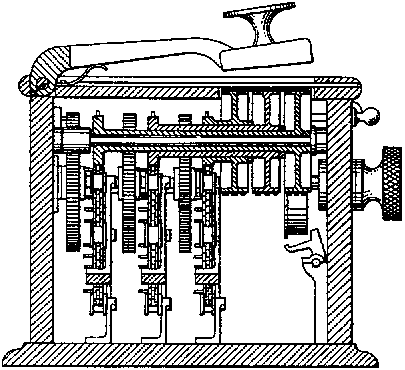
\includegraphics[scale=0.25]{images/cipher-machine.png}
    \caption{Lester Hill's patented cipher machine. It mechanically implemented a Hill cipher using a $6 \times 6$ key matrix. Under this implementation the choice of key matrix is fixed for every machine, which imaginably complicated their security.}
    \label{fig:my_label}
\end{figure}

\subsection{Hardness of Hill ciphers}

If you're not convinced of Hill ciphers' security, consider that the number of possible substitutions for a single character (using the Latin alphabet) is $26$. When substituting 2-grams for 2-grams, that number balloons to $26^2 = 676$. For 3-grams, it's $26^3 = 17576$. This exponential pattern immediately suggests that the security that a Hill cipher provides grows quickly with the dimensions of the key matrix. Even modern computers would soon run into trouble by attempting a brute-force attack where every possible substitution is tried. And so we might readily believe for now that breaking Hill ciphers should've been impossible in Lester Hill's time, when a "computer" literally meant "one who computes"; that is, people doing pen-and-paper calculations for a wage. 

\medskip
Before moving on, try meditating on whether or not this is the case. Are there potentially easier ways to break a Hill cipher, or are brute-force attacks the best we can do? 

\medskip
You might have noticed that choice of the key $k$ is rather constrained, as it must have an inverse modulo 26. Coincidentally, "HILL" is one key that does have an invertible key matrix, but there are many other $4$-letter keys, such as "MATH", that do not\footnote{"MATH" does in fact have an inverse, but only if you use the mapping $A \mapsto 1, B \mapsto 2, \dots$ instead of starting at $0$. It's rather fitting, given how mathematicians seem to prefer indices starting at $1$.}. This suggests that the keyspace of Hill ciphers is actually smaller than just the number of $m \times m$ matrices over $\mathbb{Z}_{26}$.

\medskip
Indeed, if we count the number of $m \times m$ matrices over $\mathbb{Z}_{26}$, we find that there are $26^{m^2} = 456,976$, which confirms our suspicion that a brute-force attack wouldn't be feasible. Again, this upper bound is crude because of the aforementioned constraints on the key matrix, but calculating the exact number of matrices over $\mathbb{Z}_{26}$ that are invertible modulo $26$ is far less trivial. 

\medskip
If we were to settle for a probabilistic perspective, then in choosing a matrix at random from a sample space of $m \times m$ matrices over $\mathbb{Z}_{26}$, we should expect our matrix to be invertible. Why? There are many ways we can justify this intuition, but here's one. Given that a matrix is invertible if and only if its determinant is $0$ and given that the determinant of a matrix depends on all its entries, if we had some non-invertible matrix $M$, then there's a good chance that by changing a few of its entries we could obtain a matrix $M'$ whose determinant is nonzero and is thus invertible\footnote{On top of being very loose, the analysis suffers from the fact that in practice these matrices are not chosen at random. Although the key $k$ need not be an intelligible string, often it might be, or in the very least it's likely to \textit{look} like something that's a word in our language. So the space of $m \times m$ key matrices is not random at all, since there are many constraints on what types of strings may appear in a language. To name a few: anything "word-like" in English should probably contain a vowel, and it shouldn't have many 'Z's, 'X's, or 'Q's in it either. }.

\subsection{Cracking Hill}
It turns out that the Hill cipher shares the same susceptibility to frequency analysis that the Caesar cipher has. If we knew for two plaintext digraphs what ciphertext digraphs they're mapped to, then finding the key matrix reduces to solving a system of equations. 

\medskip
For concreteness, let's return to the Jekyll-Hyde example. Let's say some adversary of Jekyll and Hyde assumed that "BL" $\mapsto$ "RC" and that "AH" $\mapsto$ "EZ". Again, this is entirely feasible through the use of frequency analysis but on digraphs instead of individual characters. For instance, we could notice that "BL" is a common digraph in English and so we could guess which digraphs in a ciphertext encrypted using a Hill cipher are most likely to correspond to "BL". This hypothetical enemy could organize the matrices \[ C = \begin{bmatrix}17 & 4 \\ 2 & 25\end{bmatrix}  \] and \[ M = \begin{bmatrix}1 & 0 \\ 11 & 7\end{bmatrix} \] and recover the key matrix by noticing that 
\begin{equation*}
    \begin{split}
            C  & = KM \\
            K & = CM^{-1}
    \end{split}
\end{equation*}
if $M$ is invertible modulo 26. In this case, it is, and $M^{-1} = \begin{bmatrix}1 & 0 \\ 17 & 5\end{bmatrix}$. You can verify for yourself that indeed \[ CM^{-1} \bmod 26 = \begin{bmatrix}7 & 8 \\ 11 & 11\end{bmatrix} \] which corresponds to the key "HILL" originally chosen by Mr. Hyde. At this point, the adversary could invert $K$ to decrypt the ciphertext and check if their assumptions were correct by seeing if the decryped text is intelligible. 

\medskip 
By knowing only two substitutions made by the $2$-dimensional Hill cipher, we can determine every substitution made by it. More generally, knowing $m$ substitutions is enough to crack an $m$-dimensional Hill cipher. The cryptanalysis behind finding these $m$ substitutions is certainly nontrivial, but for large $m$ this approach is more efficient than testing all $O(26^{m^2})$ key matrices. So while the toolkit provided by linear algebra is part of what makes Hill ciphers unique and stronger than simple substitution ciphers, the very same tools are their downfall when it comes to breaking them.

\newpage

\part{Crime and Punishment}

Hopefully by now you have made the connection between the opening example with Alice and Bob and our discussion of Hill ciphers, and perhaps you have even decrypted Alice and Bob's correspondence by yourself. For completeness' sake however, we'll treat it here as well.


\section{Revelations}
\medskip
Having just read about them, Bob is presumably using a Hill cipher to encrypt his communications with Alice. Although he and Alice haven't agreed on which cipher to use to encrypt their communications, the picture of a hill accompanying Bob's message is hopefully enough of a hint to Alice, especially since she's an avid reader of \textit{The American Mathematical Monthly}. 

\subsection{Decrypting Alice and Bob's correspondence}
We can infer that the shorter string in Bob's message
\[ \mathrm{GYBNQKURP} \]
is the key, whereas the longer string
\[ \mathrm{PIQIZAWVZZQDCCWJXTUNALNK} \]
is the ciphertext\footnote{Typically you wouldn't send the key alongside the ciphertext and just hope that an adversary won't figure out which cipher you're using. But for the sake of example we're assuming that Joe's knowledge of linear algebra is limited, which is likely for a crime boss anyway.}. The key is $9$ letters long, so the key matrix must be $3 \times 3$. Indeed $K$ here is defined as:
\[ K = \begin{bmatrix}G & Y & B \\ N & Q & K \\ U & R & P\end{bmatrix} = \begin{bmatrix}6 & 24 & 1 \\ 13 & 16 & 10 \\ 20 & 17 & 15\end{bmatrix} \]
By our algorithm, the ciphertext matrix $C_B$ for Bob's message must be $3 \times 8$ and is defined as

\begin{equation*}
    \begin{split}
        C_B & = \begin{bmatrix}P & I & W & Z & C & J & U & L \\ I & Z & V & Q & C & X & N & N \\ Q & A & Z & D & W & T & A & K \end{bmatrix} \\
        & = \begin{bmatrix}15 & 8 & 22 & 25 & 2 & 9 & 20 & 11 \\ 8 & 25 & 21 & 16 & 2 & 23 & 13 & 13 \\ 16 & 0 & 25 & 3 & 22 & 19 & 0 & 10\end{bmatrix}
    \end{split}
\end{equation*}

Recall that the ciphertext for Alice's response was 

\[ \mathrm{EKGKIIUANMOURDNFSXWTNSZQPMTLNK} \]

and so the corresponding $3 \times 10$ ciphertext matrix $C_A$  is

\begin{equation*}
    \begin{split}
        C_A & = \begin{bmatrix}E & K & U & M & R & F & W &S & P & L \\ K & I & A & O & D & S & T & Z & M & N \\ G & I & N & U & N & X & N & Q & T & K\end{bmatrix} \\
        & = \begin{bmatrix}4 & 10 & 20 & 12 & 17 & 5 & 22 & 18 & 15 & 11 \\ 10 & 8 & 0 & 14 & 3 & 18 & 19 & 25 & 12 & 13 \\ 6 & 8 & 13 & 20 & 13 & 23 & 13 & 16 & 19 & 10\end{bmatrix}
    \end{split}
\end{equation*}

Taking the inverse of $K$ modulo 26, we find that 

\[ K^{-1} \pmod{26} \equiv \begin{bmatrix}8 & 5 & 10 \\ 21 & 8 & 21 \\ 21 & 12 & 8\end{bmatrix} \]

Right multiplying $K^{-1}$ with $C_B$ modulo 26, we find that

\begin{equation*}
    \begin{split}
        K^{-1}C_B & = \begin{bmatrix}8 & 7 & 11 & 24 & 12 & 13 & 17 & 19 \\ 13 & 4 & 11 & 14 & 0 & 18 & 4 & 25\\ 19 & 0 & 4 & 13 & 8 & 19 & 4 & 25\end{bmatrix} \\
        & = \begin{bmatrix}I & H & L & Y & M & N & R & T \\ N & E & L & O & A & S & E & Z \\ T & A & E & N & I & T & E & Z\end{bmatrix}
    \end{split}
\end{equation*}

which reads as "INTHEALLEYONMAINSTREETZZ". Right multiplying $K^{-1}$ with $C_A$ modulo 26, we find that

\begin{equation*}
    \begin{split}
        K^{-1}C_A & = \begin{bmatrix}8 & 7 & 11 & 24 & 12 & 13 & 17 & 19 \\ 13 & 4 & 11 & 14 & 0 & 18 & 4 & 25\\ 19 & 0 & 4 & 13 & 8 & 19 & 4 & 25\end{bmatrix} \\
        & = \begin{bmatrix}M & S & E & C & V & W & K & N & G & T \\ E & A & R & E & E & E &D & E & E & Z \\ S & G & E & I & D & L & O & A & N & Z\end{bmatrix}
    \end{split}
\end{equation*}

which reads as "MESSAGERECEIVEDWELLDONEAGENTZZ". 

\subsection{Complications}

So it seems that Alice was able to decrypt Bob's message and send a strike force to Main Street to put an end to Joe's bootlegging operations. But is that truly the case?

\medskip
Lest we forget, Bob included the key with his message, and he had simply hoped that Joe isn't familiar with Hill ciphers. However, it's entirely possible that Joe figured out that Bob was using a Hill cipher to encrypt his message and deciphered the message. Realizing that his bootlegging operation was about to fall under, Joe might exercise a little subterfuge. He could move his bootlegging operations elsewhere and send a letter back to Bob posing as Alice to fool him into believing that his mission was successful. 

\medskip
But even if Alice and Bob had agreed on the key ahead of time, Joe could have conceivably done the same "man-in-the-middle" attack because of how Hill ciphers can be cryptanalyzed using linear algebra. Though Joe may not know anything about Hill ciphers and linear algebra, a man of his wealth could very well hire a team of mathematicians and codebreakers to break the cipher for him. Admittedly though, breaking this cipher through frequency analysis would difficult, since Bob's message is rather short and so the distribution of trigraphs in it is unlikely to reflect the broader distribution of trigraphs in English. 

\subsection{A farewell to Hill(s)}

Our digression above highlights why Hill ciphers and in general classical cryptographic ciphers are almost never used to encrypt sensitive data today. In one way or another, they are all vulnerable to clever and efficient forms of cryptanalysis. Indeed, before the modern cryptographic revolution, some practicioners of cryptography thought that there did not exist ciphers that could not be broken efficiently by through "human ingenuity"\footnote{Though mostly reputed for his literary work, Edgar Allen Poe also had an interest in cryptography. He once famously asserted that "Human ingenuity cannot concoct a cipher which human ingenuity cannot resolve", a belief that many cryptographers held before the emergence of modern cryptography.}. Today, most cryptographers don't believe this, but alas we will not give a treatment of this discussion here\footnote{If you're curious, part of the reason why we think there exists ciphers that are hard to break is because of the belief that one-way functions exist. Roughly speaking, one-way functions are those that are easy for a computer to compute but  whose their inverses are hard to compute. That is, calculating $f(x)$ for some input $x$ is easy, but finding the preimage $x$ of $f(x)$ is hard. Such functions have great applicability for creating ciphers, but we don't know for sure that they exist. There are reasons to be believe that they do, which are covered in better detail in books on theoretical computer science or cryptography.}.

\medskip
But despite its problems, the Hill cipher readily exemplifies just how much cryptography draws from different areas in mathematics, and we hope this short exploration of them has convinced you of this. And if not, hopefully the tribulations of Dr. Jeykll and Mr. Hyde and of Alice and Bob have at least entertained you along the way.

\end{document}
